\begin{figure*}[ht]
\centering
\begin{minipage}[t]{0.3\textwidth}
    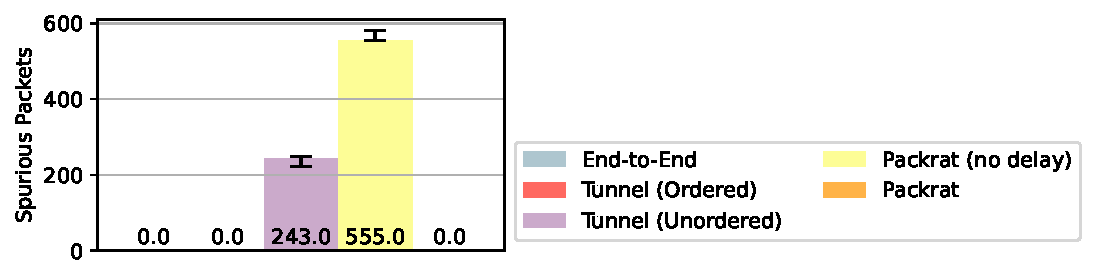
\includegraphics[width=\linewidth, trim=245 15 5 65, clip]{packrat/figures/spurious_retx_legend.pdf}
    \begin{subfigure}[b]{\linewidth}
        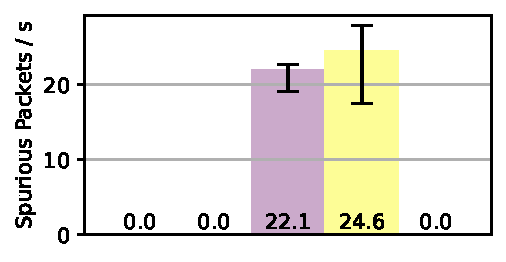
\includegraphics[width=\linewidth]{packrat/figures/spurious_retx_http.pdf}
        \caption{HTTP/3 download.}
        \label{fig:packrat:spurious:http}
    \end{subfigure}
    \begin{subfigure}[b]{\linewidth}
        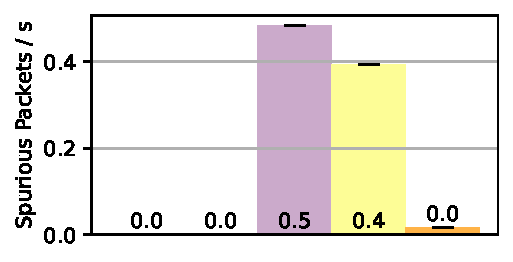
\includegraphics[width=\linewidth]{packrat/figures/spurious_retx_media.pdf}
        \caption{Low-latency media.}
        \label{fig:packrat:spurious:media}
    \end{subfigure}
    \caption{The unordered tunnel and Packrat without modifying the end-to-end
     reorder delay cause the client to receive spurious retransmissions.
     Adding a reorder delay with Packrat significantly reduces them.}
    \label{fig:packrat:spurious}
\end{minipage}%
\hfill
\begin{minipage}[t]{0.68\textwidth}
    \centering
    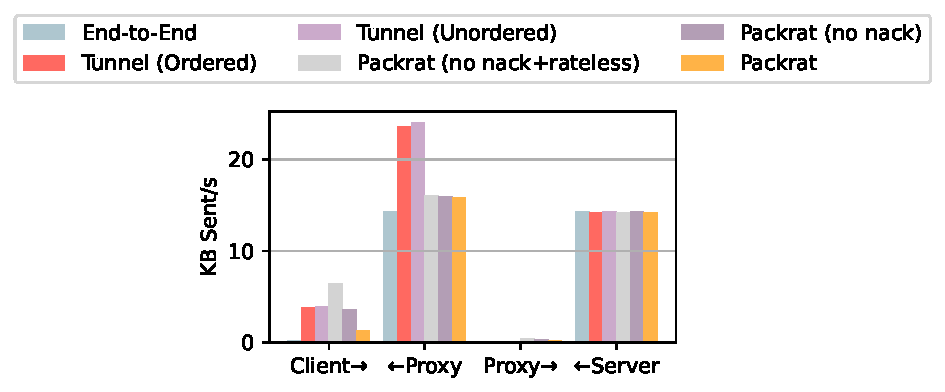
\includegraphics[width=0.9\linewidth, trim=5 140 5 5, clip]{packrat/figures/network_stats_media_legend.pdf}
    
    \begin{subfigure}[b]{0.48\linewidth}
        \centering
        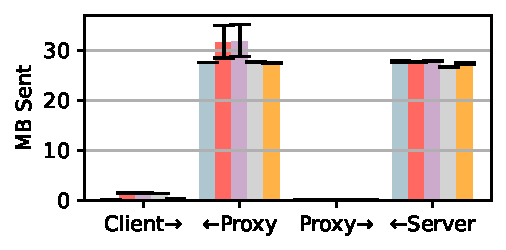
\includegraphics[width=\linewidth]{packrat/figures/network_stats_http_tx_bytes.pdf}
        \caption{HTTP/3 download (bytes).}
        \label{fig:packrat:link-overheads:http-bytes}
    \end{subfigure}
    \begin{subfigure}[b]{0.51\linewidth}
        \centering
        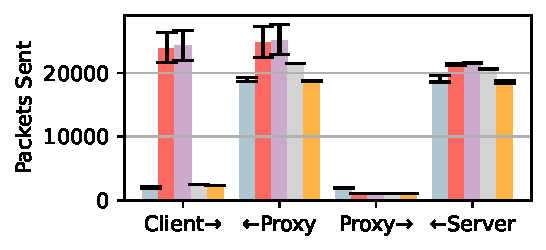
\includegraphics[width=\linewidth]{packrat/figures/network_stats_http_tx_packets.pdf}
        \caption{HTTP/3 download (packets).}
        \label{fig:packrat:link-overheads:http-packets}
    \end{subfigure}\\

    \begin{subfigure}[b]{0.49\linewidth}
        \centering
        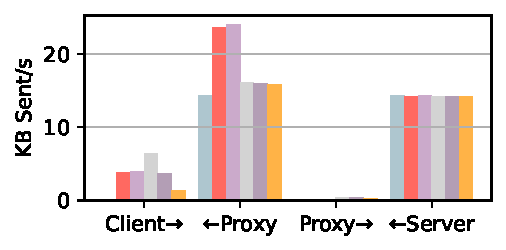
\includegraphics[width=\linewidth]{packrat/figures/network_stats_media_tx_bytes.pdf}
        \caption{Low-latency media (bytes).}
        \label{fig:packrat:link-overheads:media-bytes}
    \end{subfigure}
    \begin{subfigure}[b]{0.49\linewidth}
        \centering
        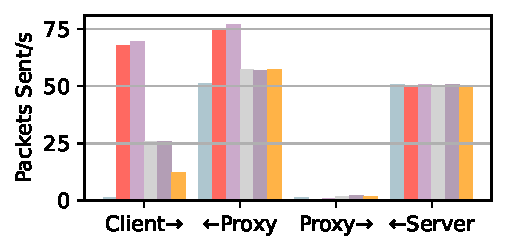
\includegraphics[width=\linewidth]{packrat/figures/network_stats_media_tx_packets.pdf}
        \caption{Low-latency media (packets).}
        \label{fig:packrat:link-overheads:media-packets}
    \end{subfigure}
    
    \caption{The number of bytes (left) and packets (right) sent between the
     client, proxy, and server. The statistics are captured directly from the
     network interface. The link overheads from quACKs using the Packrat proxy are
     comparable to those of the underlying acknowledgment scheme. The client
     sends fewer bytes with rateless quACKs, and fewer packets with sparse
     quACKing. The tunnel aggressively ACKs and retransmits.}
    \label{fig:packrat:link-overheads}
\end{minipage}
\end{figure*}